% Appendix A

\chapter{} % Main appendix title

\label{AppendixA} % For referencing this appendix elsewhere, use \ref{AppendixA}

\lhead{Apéndice} % This is for the header on each page - perhaps a shortened title

Algunas cosas interesantes que faltó incluir en el trabajo:
Primero una imagen de algunas versiones de MODI, que fueron posibles por tener acceso a impresoras 3D ya que hacen muy simple el proceso de hacer cambios en los prototipos.

\begin{figure}[htbp]
	\centering
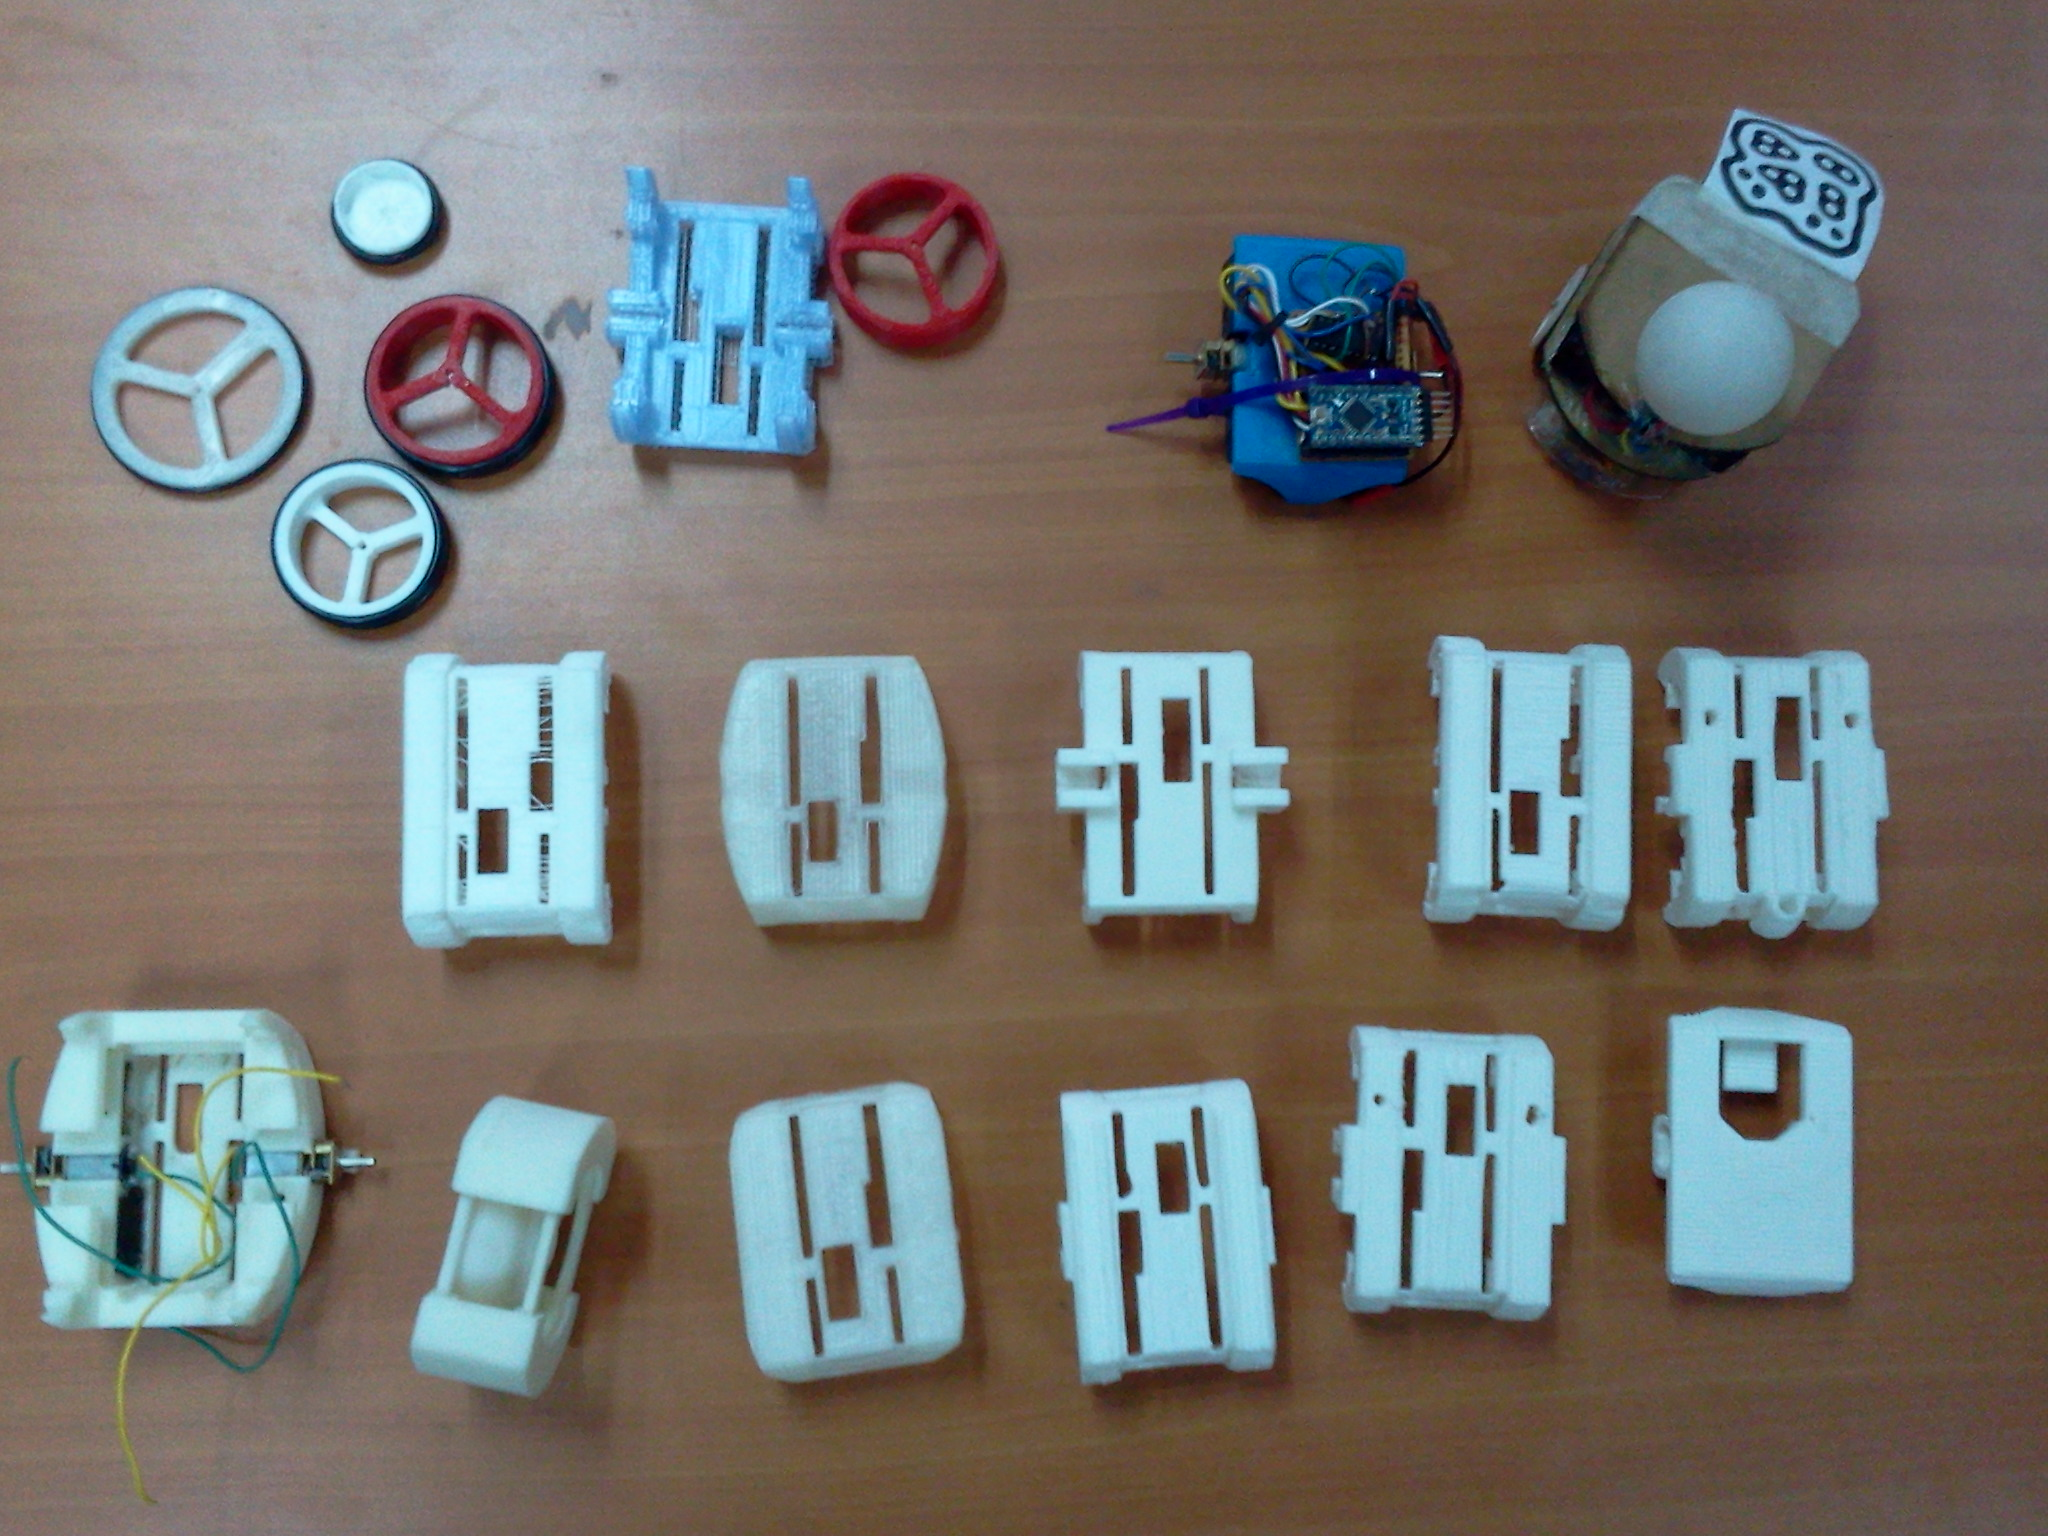
\includegraphics[width=\textwidth]{./Pictures/historia.jpg}
		\rule{35em}{0.5pt}
	\caption[Historia de construcción]{Algunos de los modelos que se construyeron para llegar a la versión final de MODI.}
	\label{fig:Historia}
\end{figure}

\newpage 
Lo segundo es el PCB diseñado para MODI que une el controlador de motores al arduino FIO y permite contectar un LED RGB.
\begin{figure}[htbp]
	\centering
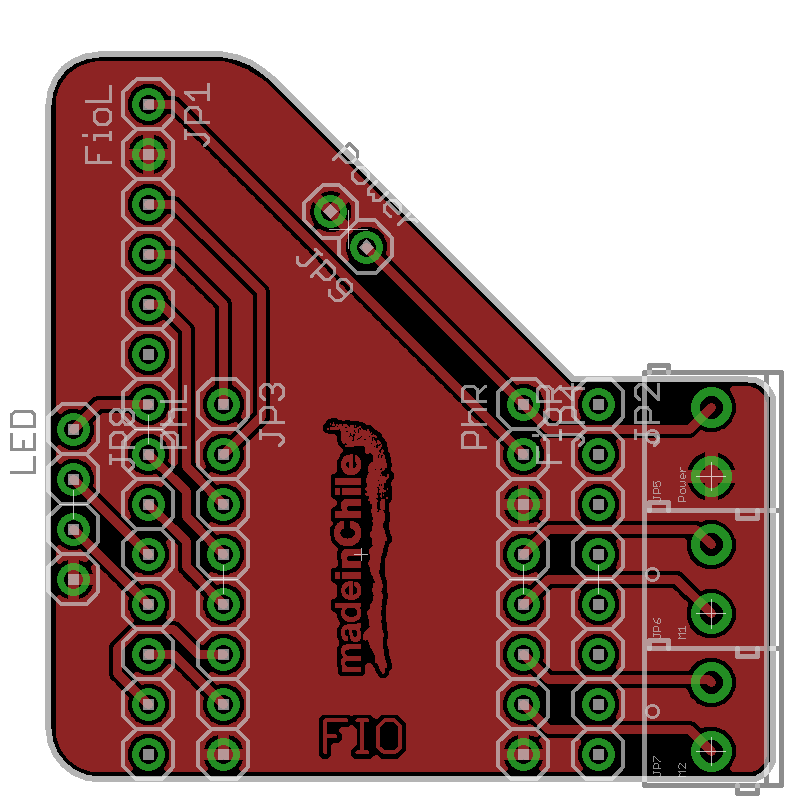
\includegraphics[width=\textwidth]{./Figures/MODI/pcbmodi.png}
		\rule{35em}{0.5pt}
	\caption[PCB MODI]{PCB diseñada para conectar motores, LED RGB al Arduino FIO.}
	\label{fig:PCBA}
\end{figure}
